%\documentclass[english]{beamer}
\documentclass[english,hangout]{beamer}
%\documentclass[aspectratio=169]{beamer}
%\usepackage{amsmath}
%\usepackage{amssymb}
\usepackage{rotating}
\usepackage{verbatim}
\usepackage{latexsym}
\usepackage{graphicx}
\usepackage{tabularx}
\usepackage{ragged2e}
\usepackage{eurosym}   % Euro symbol: \euro
\usepackage{listings}
\usepackage{multirow}
\usepackage{colortbl}
\usepackage{textcomp}  % many special symbols
\usepackage{lmodern}
\usepackage{times}
\usepackage[T1]{fontenc}
\usepackage[utf8]{inputenc}
\usepackage[english]{babel}
\usepackage{booktabs}


%\usetheme[fb2]{FrankfurtUniversity}
\usetheme[fb2,noslogan]{FrankfurtUniversity}
%\slogan{\large\color{red}UNAUTHORIZED}


\title{Blockchain Solution to\\Healthcare Record System using\\Hyperledger Fabric}
\subtitle{Sprint 1 review}
\author{Jathin Sreenivas, Kshitij Yelpale, Varsha Vasudev Kamath}
%\institute{Frankfurt University of Applied Sciences\\}
\date{\today}%{November 24, 2020}


\begin{document}


\begin{frame}
\titlepage
\end{frame}
%\addtocounter{framenumber}{-1}



\begin{frame}
   \frametitle{Agenda}
   \tableofcontents%[hideallsubsections]
\end{frame}




\section{Sprint 1}

\subsection{Results}

\begin{frame}[fragile]
 \frametitle{Sprint 1}
 \framesubtitle{Results - Overview}
  \begin{itemize}
    \item Understanding on how Hyperledger Fabric can be used to solve the problem.
    \item Architecture.
    \item Understanding of the scenario.
    \item Creation of a basic network on hyperledger fabric.
    \item Deploying a chaincode.
    \item Pending : Data Security
  \end{itemize}
\end{frame}

\subsection{Architecture}

\begin{frame}[fragile]
  \frametitle{Architecture}
\begin{center}
        \vspace{-1.2em}
            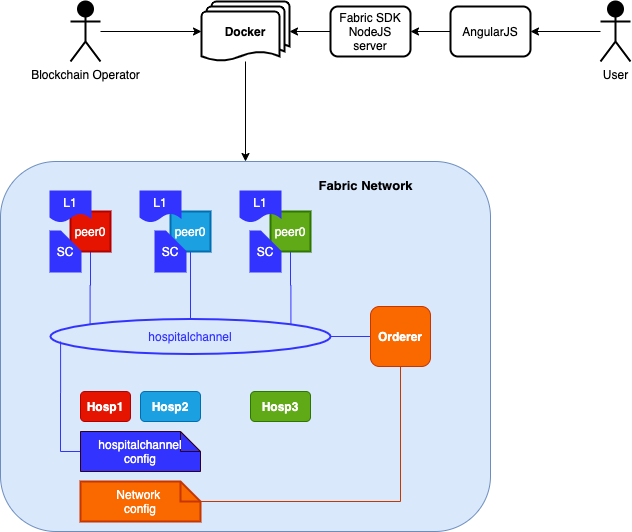
\includegraphics[height=6cm]{Architecture_v2.png}
        \end{center}
        \vspace{-3mm}
\end{frame}


\subsection{Activity Diagrams}

\begin{frame}
  \frametitle{Activity Diagrams}
\begin{center}
        \vspace{-1.2em}
            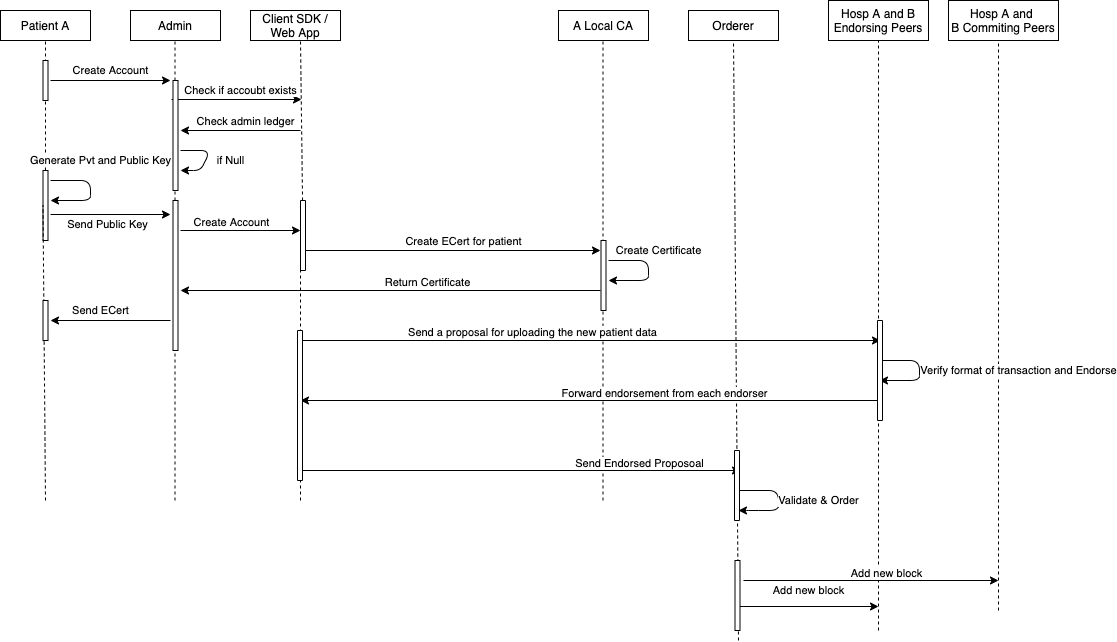
\includegraphics[height=6cm]{first.png}
        \end{center}
        \vspace{-3mm}

\end{frame}

\begin{frame}
  \frametitle{Activity Diagrams}
\begin{center}
        \vspace{-1.2em}
            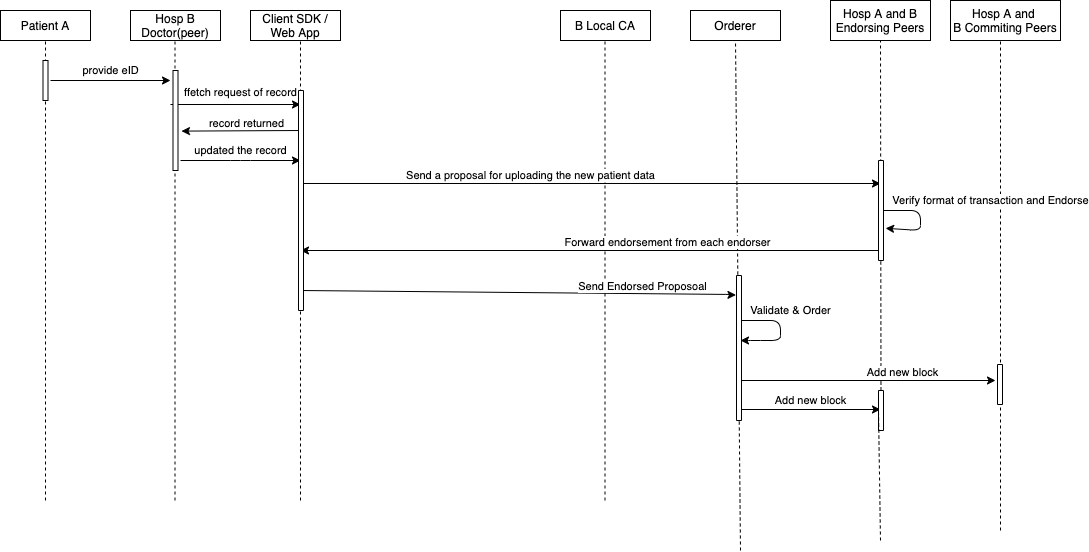
\includegraphics[height=6cm]{second.png}
        \end{center}
        \vspace{-3mm}

\end{frame}

\subsection{User Cases}

\begin{frame}
    \frametitle{Use Cases 1/2}
    \begin{itemize}
        \item Each organization has an admin peer which has rights of creating patient's record in blockchain, add new peer in hospital and adding new organization in the channel only if that admin belongs to an organization present in Channel configuration.
        \item Patient, doctor and admin screen on UI acts as the client.
        \item Patient's record information will come through any organization peer (will keep one default organization in channel configuration).
        \item Doctor can see a list of all available patients' information and can add medication steps for a patient. To fetch patients' info for doctors, doctor needs to specify the hospital and peer which he belongs to at the time of login.
    \end{itemize}
\end{frame}

\begin{frame}
    \frametitle{Use Cases 2/2}
    \begin{itemize}
        \item When a doctor makes any change and make a proposal, the endorsement request will be sent to all endorsing peers. As per endorsement policy, we will keep 51\% (PBFT) approval criteria for endorsement request.
        \item Admin will create new patient on the blockchain network after taking patient's public key and provide patient id and certificate in return which can be used to fetch patient's information.
        \item We will design more security aspects after more deep research and integrate in Sprint 3.
    \end{itemize}
\end{frame}


\subsection{Demo}

\begin{frame}[fragile]
 \frametitle{Sprint 1}
    \begin{center}
        \vspace{-1.2em}
            Demo
        \end{center}
%\tiny Source: \texttt{https://hyperledger-fabric.readthedocs.io/en/latest/txflow.html}
\end{frame}

\subsection{Tasks Overview}

\begin{frame}[fragile]
 \frametitle{Sprint 1}
 \framesubtitle{Tasks}
    \begin{center}
        \vspace{-1.2em}
            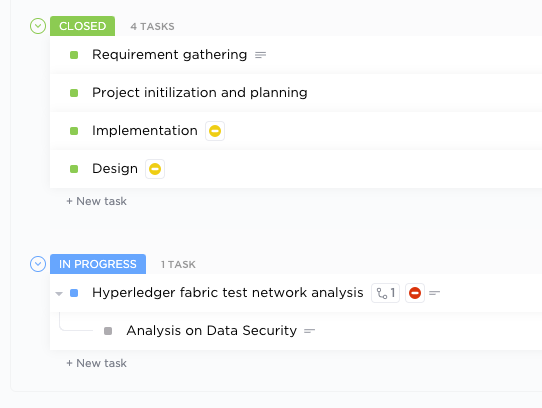
\includegraphics[height=6cm]{Sprint1Results.png}
        \end{center}
%\tiny Source: \texttt{https://hyperledger-fabric.readthedocs.io/en/latest/txflow.html}
\end{frame}


\section{Sprint 2}

\subsection{Project Plan}

\begin{frame}[fragile]
 \frametitle{Sprint 2}
 \framesubtitle{Tasks}
    \begin{center}
        \vspace{-1.2em}
            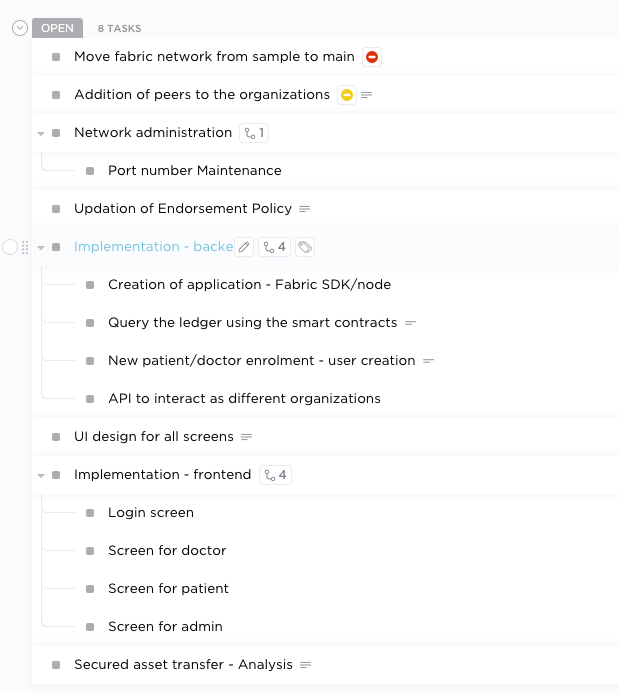
\includegraphics[height=6cm]{Sprint2Tasks.png}
        \end{center}
        \vspace{-3mm}
%\tiny Source: \texttt{https://hyperledger-fabric.readthedocs.io/en/latest/txflow.html}
\end{frame}



\section{References}

\begin{frame}
\frametitle{References}
\begin{thebibliography}{00}
\bibitem{b1} https://www.ncbi.nlm.nih.gov/pmc/articles/PMC7010942/
\bibitem{b2} https://www.ncbi.nlm.nih.gov/pmc/articles/PMC7474412/
\bibitem{b3} https://www.sciencedirect.com/science/article/pii/S2214212619306155
\bibitem{b4} https://hyperledger-fabric.readthedocs.io/ Accessed-On:01/12/2020
\bibitem{b5} https://medium.com/@lichunshen84/build-a-blockchain-poc-application-using-hyperledger-fabric-5a32687072b7, Accessed-On:01/12/2020
\end{thebibliography}

\end{frame}




\end{document}